\section{Design}
\label{sec:ldu}

%$$$$$$$$$$$$$$$$$$$$$$$$$$$$$$$$$$$$$$$$$$$$$$$$$$$$$$$$$$$$$$$$$$$$$$$$$$$$$$$$
%Paragraph 1: LDU의 특징을 간단한 설명과 이번장에 대한 설명(LDU의 특징을 요약하여 설명)
%$$$$$$$$$$$$$$$$$$$$$$$$$$$$$$$$$$$$$$$$$$$$$$$$$$$$$$$$$$$$$$$$$$$$$$$$$$$$$$$$

The \LDU is a log-based concurrent update method to remove scalability
bottlenecks for the update-heavy data structure.
The \LDU further improves the performance scalability for update-heavy data structures
by eliminating the synchronized time-stamp management overhead from previous
research. One additional advantage of using the \LDU is that it reuses the log
slots already allocated and used by preceding operations.
%The previous research using the synchronized time-stamp counters method may incur
%time-stamp merging and ordering overhead.
%The \LDU can solve these sequential processing by using two techniques.
%The \LDU instantly removes operation logs at update time that requires time-stamp
%counter and reuses the garbage log instead of creating a new log
%thereby eliminating the synchronized time-stamp counter and cache communication
%bottleneck.
This section explains these algorithmic design aspects of the \LDU.

\subsection{Approach}


%$$$$$$$$$$$$$$$$$$$$$$$$$$$$$$$$$$$$$$$$$$$$$$$$$$$$$$$$$$$$$$$$$$$$$$$$$$$$$$$$
%Paragraph 2: timestamp가 필요한 이유 : time-sensitive update operation log.
%$$$$$$$$$$$$$$$$$$$$$$$$$$$$$$$$$$$$$$$$$$$$$$$$$$$$$$$$$$$$$$$$$$$$$$$$$$$$$$$$
The fundamental reason for requiring synchronized time-stamp counters is that some
operations need to be ordered.
For example, a process logs an insert operation to the per-core memory, then
it migrates to another core, and it logs a remove operation, which must eventually
execute after the insert operation~\cite{SilasBoydWickizerPth}.
%Thus, the synchronized time-stamp counters are needed.
To specifically explain a time-sensitive log, we use the symbol label used by
this paper~\cite{Clements15SCR}.
We describe insert as plus-circles $\oplus$, remove as minus-circles
$\ominus$ and object as color-circles \inv{2}{B}(object B). 
Color and vertical offset differentiate cpus.
For example
\begin{center}
$\oplus$\inv{1}{A}, $\oplus$\inv{2}{B}, $\oplus$\inv{3}{C},$\ominus$\inv{2}{A},
$\ominus$\inv{3}{C}, $\oplus$\inv{3}{A}, $\oplus$\inv{3}{C},$\ominus$\inv{1}{C}
\end{center}
consists of five insert operations, three remove operation, three cpus, and
three objects.
This example shows that $\oplus$\inv{1}{A} and $\ominus$\inv{2}{A},
time-sensitive logs, must be executed in chronological order.
The \LDU can eliminate this time-sensitive logs at update time;as a result, the synchronized time-stamp counters are eliminated.
One more important fact that these time-sensitive operation logs may be removed
by optimization phase.
For example, insert-remove operations or remove-insert operations, 
$\oplus$\inv{1}{A}$\ominus$\inv{2}{A}, $\oplus$\inv{3}{C}$\ominus$\inv{3}{C} 
and $\oplus$\inv{3}{C}$\ominus$\inv{1}{C}, are the cancelable operations before
a reader, so the remained operation logs, 
\begin{center}
 $\oplus$\inv{2}{B}, $\oplus$\inv{3}{A}
\end{center}
, are non-time-sensitive logs.
When update operations occur, the \LDU removes these time-sensitive logs using
the update-side removing technique.

%$$$$$$$$$$$$$$$$$$$$$$$$$$$$$$$$$$$$$$$$$$$$$$$$$$$$$$$$$$$$$$$$$$$$$$$$$$$$$$$$
%Paragraph 3:  time-sensitive update operation 삭제 방법: Update-side Abosrbing 
%$$$$$$$$$$$$$$$$$$$$$$$$$$$$$$$$$$$$$$$$$$$$$$$$$$$$$$$$$$$$$$$$$$$$$$$$$$$$$$$$

To remove the time-sensitive log, the \LDU uses the update-side removing scheme.
When insert-remove operations occur in terms of the same object, the scheme removes the insert-remove operations at update time.
The OpLog also optimizes by removing the existing operation rather than
adding the new one, but the OpLog can not remove log when a thread 
migrates other core, so it needs additional sequential processing during
the optimization phase.
The \LDU, however, has no problem with the migrating other core during logging
process because it uses the shared atomic swap operation in an individual object.

%$$$$$$$$$$$$$$$$$$$$$$$$$$$$$$$$$$$$$$$$$$$$$$$$$$$$$$$$$$$$$$$$$$$$$$$$$$$$$$$$
%Paragraph 5: 리눅스의 Update-side removing 수행 방법
%$$$$$$$$$$$$$$$$$$$$$$$$$$$$$$$$$$$$$$$$$$$$$$$$$$$$$$$$$$$$$$$$$$$$$$$$$$$$$$$$
The update-side removing logs scheme performs an atomic swap operation in an
individual object for shared memory systems.
This atomic swap operation allows update operations to atomically remove with the
previous cancelable log.
To achieve update-side removing log, 
first, add the mark field to the individual object
structure then use it as a status flag. 
For example, consider the insert-remove operation sequence at the same object.
The first insert operation marks the mark field and then it logs into the queue.
If the remove operation occur, the \LDU will not logs;it only changes the mark field.
When the reader applies logs, the \LDU applies the logs to the original data
structure in case of the true value of the mark field.
The benefit of this update-side removing scheme is twofold:not only it can
eliminate the time-sensitive operation but also it can cancel the previous
operation log in the queue.

%$$$$$$$$$$$$$$$$$$$$$$$$$$$$$$$$$$$$$$$$$$$$$$$$$$$$$$$$$$$$$$$$$$$$$$$$$$$$$$$$
%Paragraph 7: 또 최적화 방법 reusing garbage object : 
%$$$$$$$$$$$$$$$$$$$$$$$$$$$$$$$$$$$$$$$$$$$$$$$$$$$$$$$$$$$$$$$$$$$$$$$$$$$$$$$$

The second technique, called reusing garbage logs, reuses the garbage log
instead of creating a new log.
The garbage log is the log that has been already cancelled by 
using the update-side removing scheme,
but it still occupies a slot in the queue.
For example, consider the insert-remove-insert operations.
After the second remove operation, the log is remaining in the queue, but it has been
already cancelled by using update-side removing; hence {\it insert} mark field
is zero in the queue.
In this case, the third insert operation reuses the log in the queue instead of 
creating a new log using the atomic swap, so it can reduce not only the memory
overhead but also the queuing overhead.

%$$$$$$$$$$$$$$$$$$$$$$$$$$$$$$$$$$$$$$$$$$$$$$$$$$$$$$$$$$$$$$$$$$$$$$$$$$$$$$$$
%Paragraph 11: 중간에 한번씩 log를 flush
%$$$$$$$$$$$$$$$$$$$$$$$$$$$$$$$$$$$$$$$$$$$$$$$$$$$$$$$$$$$$$$$$$$$$$$$$$$$$$$$$
In addition to the update-side removing logs and the reusing garbage logs,
the \LDU uses the previous research's scheme that periodically applies the operation logs 
to reduce memory usage and to keep the log from growing without end.
This approach is similar with the method of previous research such as the OpLog's
batching updates and flat combining(FC)'s combiner thread.

%$$$$$$$$$$$$$$$$$$$$$$$$$$$$$$$$$$$$$$$$$$$$$$$$$$$$$$$$$$$$$$$$$$$$$$$$$$$$$$$$
%Paragraph 8: LDU의 로그는 두 종류의 queue에 저장할 수 있도록 지원
%$$$$$$$$$$$$$$$$$$$$$$$$$$$$$$$$$$$$$$$$$$$$$$$$$$$$$$$$$$$$$$$$$$$$$$$$$$$$$$$$
Furthermore, we design a log's queue using both the per-core and the global queue
to further support various data structures.
The per-core queue of the \LDU can remove CAS operations, which access global
head pointer. 
However, the per-core queue does not properly apply to all data structures since
it has some drawbacks.
The per-core queue has a memory overhead, and developers may need
an additional management code for per-core memory management(see section~\ref{sec:linux}).
To overcome these shortcomings, the \LDU also supports a global queue.
The global queue of the \LDU is simple and easy to apply, so it can easily use any
data structure.
Though global queue can not perfectly remove global CAS operations, it can
mitigate the cache communication overhead by using update-side removing
logs and by reusing garbage logs because it reduces the number of inserting the
queue(see section~\ref{sec:evaluation}-B).

%$$$$$$$$$$$$$$$$$$$$$$$$$$$$$$$$$$$$$$$$$$$$$$$$$$$$$$$$$$$$$$$$$$$$$$$$$$$$$$$$
%Paragraph 9: log를 저장하는 queue의 종류는 non-blocking queue를 사용
%$$$$$$$$$$$$$$$$$$$$$$$$$$$$$$$$$$$$$$$$$$$$$$$$$$$$$$$$$$$$$$$$$$$$$$$$$$$$$$$$
The \LDU uses the non-blocking queue regardless of the per-core queue or the
global queue since it can proceed without any lock.
Among non-blocking queues, the \LDU uses multiple producers and single consumer
based non-blocking queue thereby reducing the CAS operations.
This queue always inserts node where is a first pointer, so it can minimize
iteration loops because it causes another CAS operation.
In addition, this queue merely considers single consumer when it applies
the logs, so it does not need complex algorithms for the remove operation.
The queue uses atomic swap operation to acquire all operation logs.

\subsection{Example}
\begin{figure*}[h]
  \begin{center}
     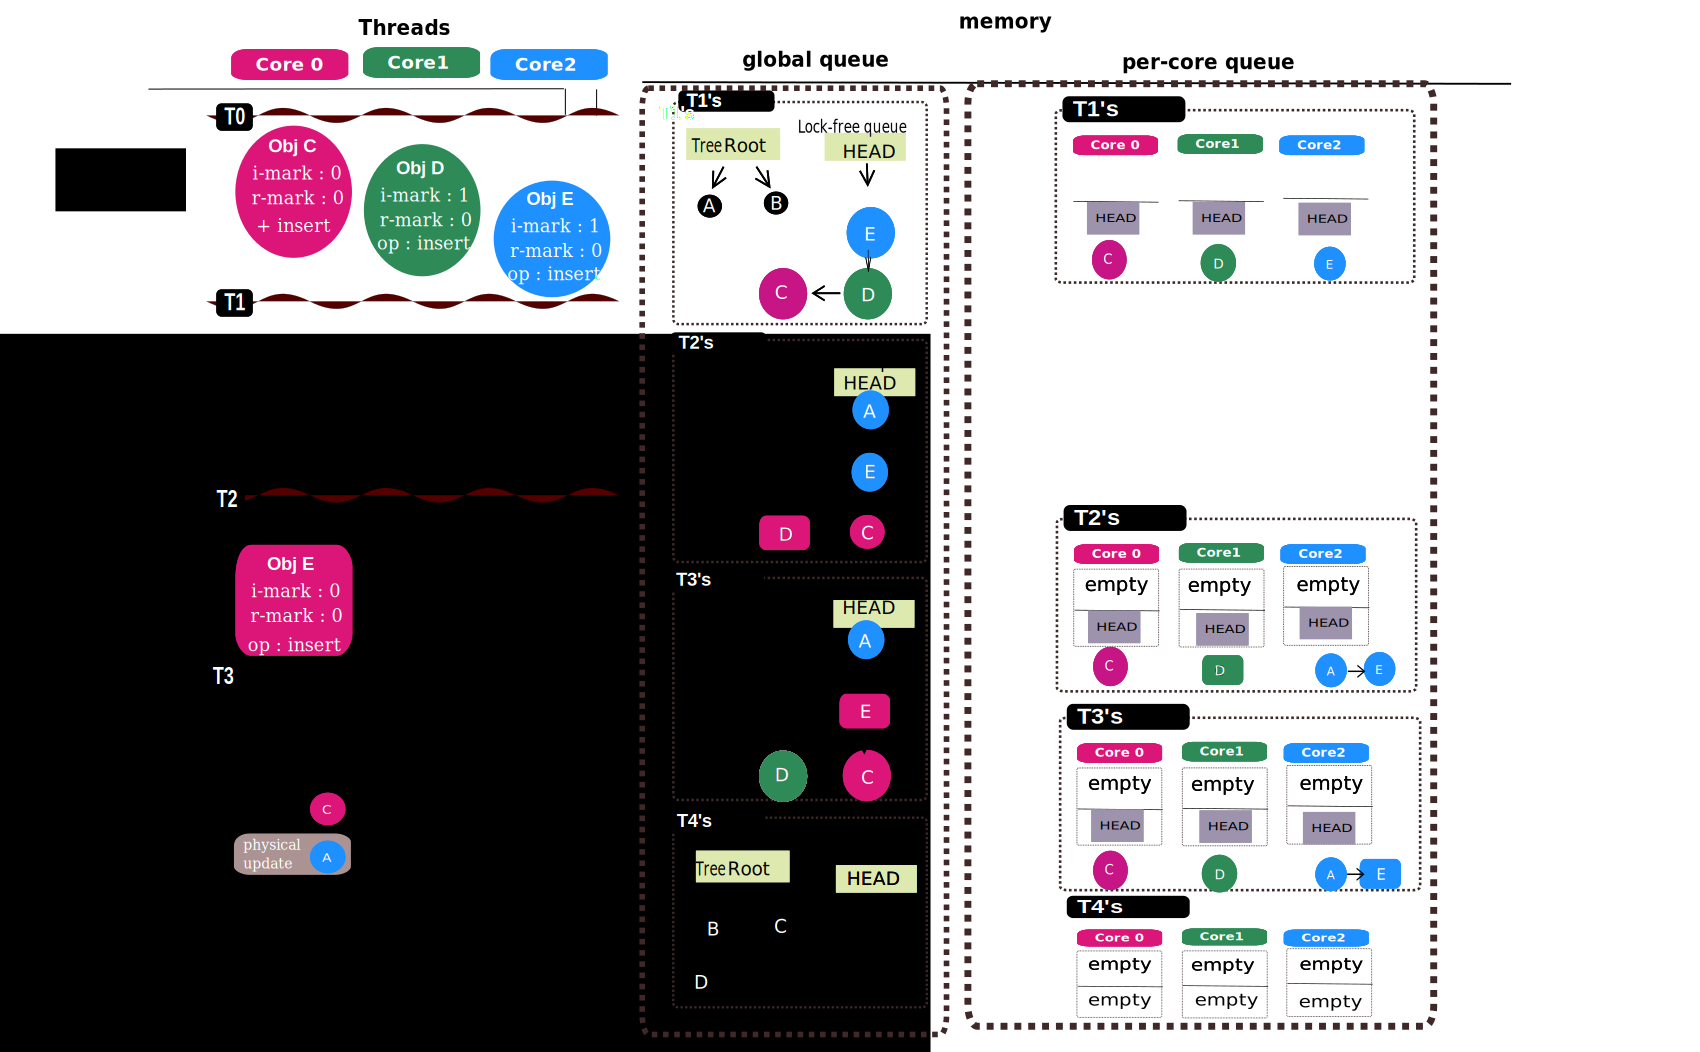
\includegraphics[width=1.0\textwidth,height=0.4\textheight]{fig/basic_gldu}
  \end{center}
  \caption{The \LDU example showing seven update operations(insert C, insert D ,
  insert E, remove D, insert A, insert D, and remove E) and one read
  operation. The execution flows from top to bottom.
  Memory represents original data structure and logging queue at T1, T2, T3 and T4,
  respectively. The initial tree data structure contains two object, A and B , and the queue is empty.
  The seven update operations concurrently execute without locks and a single
  reader executes with lock.}
  \label{fig:basic}
\end{figure*}

%$$$$$$$$$$$$$$$$$$$$$$$$$$$$$$$$$$$$$$$$$$$$$$$$$$$$$$$$$$$$$$$$$$$$$$$$$$$$$$$$
%Paragraph 1: Flowchart 구조 설명 
%$$$$$$$$$$$$$$$$$$$$$$$$$$$$$$$$$$$$$$$$$$$$$$$$$$$$$$$$$$$$$$$$$$$$$$$$$$$$$$$$

Figure \ref{fig:basic} shows an example of the \LDU with a per-core queue and
a global queue.
In order to explain the concurrent deferred update method for the update-heavy
data structure, we show how seven update operations can concurrently execute
without lock before the read operation.
The update operations sequence is
\begin{center}
$\oplus$\inv{1}{C}, $\oplus$\inv{2}{D}, $\oplus$\inv{3}{E},$\ominus$\inv{1}{D},
$\ominus$\inv{3}{A}, $\oplus$\inv{2}{D}, $\ominus$\inv{1}{E}. 
\end{center}.
To explain the \LDU, we use the previously used symbols with a new garbage symbol as
rectangle \res{1}{D}.
In this figure, execution flows from top to bottom.
The left side of figure shows cpu operations, and the right side of figure shows data structures
contents at a particular time in a memory.
Initially, the tree data structure contains \inv{0}{A} and \inv{0}{B}, and 
the queue is empty.

%$$$$$$$$$$$$$$$$$$$$$$$$$$$$$$$$$$$$$$$$$$$$$$$$$$$$$$$$$$$$$$$$$$$$$$$$$$$$$$$$
%Paragraph 2: Flowchart 그림 설명 
%$$$$$$$$$$$$$$$$$$$$$$$$$$$$$$$$$$$$$$$$$$$$$$$$$$$$$$$$$$$$$$$$$$$$$$$$$$$$$$$$
In the top of figure, \code{Core1}, \code{Core2} and \code{Core3} perform the
concurrent update operations, $\oplus$\inv{1}{C}, $\oplus$\inv{2}{D} and
$\oplus$\inv{3}{E}, without lock.
Since the \LDU uses non-blocking queue to save the operation logs, this step does not need
a update lock, so all threads can be executed in parallel without any lock contention.
At \code{T1}, the tree contains objects \inv{0}{A} and \inv{0}{B}. 
The per-core queue and the global queue contain $\oplus$\inv{1}{C}, $\oplus$\inv{2}{D} and
$\oplus$\inv{3}{E}, but the logs in the per-core queue are separated.

The next operations are $\ominus$\inv{1}{D} and $\ominus$\inv{3}{A}.
When the $\ominus$\inv{1}{D} operation is executed, the \LDU atomically changes 
the mark field in the object instead of inserting the queue.
Then, $\ominus$\inv{3}{A} inserts the queue because it is a new operation log.
At \code{T2}, the per-core queue and the global queue contain 
$\oplus$\inv{1}{C}, $\oplus$\res{2}{D}, $\oplus$\inv{3}{E} and
$\ominus$\inv{3}{A}.
The insert mark field in the object \res{2}{D} is false, called a garbage object, 
has remained in the queue, but it was already canceled 
by update-side removing logs.

The last operations are $\oplus$\inv{2}{D}, $\ominus$\inv{1}{E}.
The \LDU reuses the log in the queue instead of 
creating a new log using atomic swap.
Thus, the object \res{2}{D} changes \inv{2}{D}, and then the object \inv{3}{E} 
changes \res{3}{E} by performing the update-side removing logs scheme.
At \code{T3}, per-core queue contains
$\oplus$\inv{1}{C}, $\oplus$\inv{2}{D}, $\ominus$\inv{3}{A} 
and $\oplus$\res{3}{E}.

Before the read function, it need to lock the original tree lock using the
exclusive lock in order to protect the tree operations.
The \LDU migrates from queue to tree, each of which is the marked object.
Thus, $\oplus$\inv{1}{C}, $\oplus$\inv{2}{D} and $\ominus$\inv{3}{A} are
migrated except for the $\oplus$\res{3}{E} a garbage log.
At T5, the tree contains \inv{0}{B}, \inv{0}{C} and
\inv{0}{D}, so finally, the reader can read eventually consistent data.


\begin{figure*}[h]
\begin{center}
\inputminted[linenos,fontsize=\footnotesize, tabsize=2]{c}{src/ldu_logical_a.c}
\end{center}
\caption{The \LDU concurrent insert algorithm.  This logging may be called by
original update functions without locks. The concurrent update functions are
divided into three phase.}
\label{fig:gldulogicalupdate}
\end{figure*}


\begin{figure*}[h]
\begin{center}
\inputminted[linenos,fontsize=\footnotesize, tabsize=2]{c}{src/ldu_logical_b.c}
\end{center}
\caption{The \LDU concurrent remove algorithm.}
\label{fig:gldulogicalupdate}
\end{figure*}


\subsection{The Algorithm and Correctness}

This section shows skeleton of an algorithm.
We exclude the log's queue and the \LDU's detailed data structures for
exposition simplicity.

\subsubsection{inserting logs}
%$$$$$$$$$$$$$$$$$$$$$$$$$$$$$$$$$$$$$$$$$$$$$$$$$$$$$$$$$$$$$$$$$$$$$$$$$$$$$$$$
%Paragraph 1:LDU Concurrent Updates 알고리즘 코드 및 설명 
%$$$$$$$$$$$$$$$$$$$$$$$$$$$$$$$$$$$$$$$$$$$$$$$$$$$$$$$$$$$$$$$$$$$$$$$$$$$$$$$$
Figure \ref{fig:gldulogicalupdate} shows concurrent update functions.
The concurrent update functions are divided into three phase.
The first phase checks this object to see whether or not the
object is a cancelable object(Line 4, 20).
When this code is executed, the \code{synchronize} function can
be invoked by a reader or a periodic timer, so phase 1 needs the atomic operation.
If the corresponding mark field is true, then its mark field is changed to false.
In phase 2 checks this log to see weather or not has already inserted in
the queue(Line 8, 24).
If so, because mark field is marked(Line 6, 22), this function directly returns
true.
In the last phase, the operation log inserts the non-blocking queue
when the operation log is the first used log(Line 12, 28).

%$$$$$$$$$$$$$$$$$$$$$$$$$$$$$$$$$$$$$$$$$$$$$$$$$$$$$$$$$$$$$$$$$$$$$$$$$$$$$$$$
%Paragraph 4: 리눅스의 update operation의 특징을 이용한 Update-side Abosrbing 
%$$$$$$$$$$$$$$$$$$$$$$$$$$$$$$$$$$$$$$$$$$$$$$$$$$$$$$$$$$$$$$$$$$$$$$$$$$$$$$$$
This algorithm is correct because Linux kernel has a unique update
operations sequence.
For example, if an insert operation occur, then next operation must be a remove
operation at the same object because the kernel's update function
is separated from search, alloc and free functions.
The remove-remove or insert-insert operation in Linux kernel is
forbidden: if remove-remove operation occur, the second remove operation may
encounter a crash because this object can be concurrently freed after the first remove
operation, so we check the corresponding mark field(Line 5, 21).

\subsubsection{applying logs}

\begin{figure*}[h]
\begin{center}
\inputminted[linenos,fontsize=\footnotesize, tabsize=2]{c}{src/ldu_physical.c}
\end{center}
%\rule{\columnwidth}{0.5pt}
%\vspace{-\baselineskip}
\caption{The \LDU applying logs algorithm. The \code{synchronize\_ldu} may be
 called by a reader or a timer handler and converts logs to original data structure
 traversing the log's queue.}
\label{fig:glduphysicalupdate}
\end{figure*}


%$$$$$$$$$$$$$$$$$$$$$$$$$$$$$$$$$$$$$$$$$$$$$$$$$$$$$$$$$$$$$$$$$$$$$$$$$$$$$$$$
%Paragraph 2:LDU Deferred Updates 알고리즘 코드 및 설명 
%$$$$$$$$$$$$$$$$$$$$$$$$$$$$$$$$$$$$$$$$$$$$$$$$$$$$$$$$$$$$$$$$$$$$$$$$$$$$$$$$

Figure \ref{fig:glduphysicalupdate} shows deferred update function, which
applies the operation logs.
The \code{synchronize} function is invoked before the read, or it can be
periodically invoked by the timer handler because of preventing the continuous
growing the logs.
Before the execution of the \code{synchronize} function, it has been locked by using
the object lock, so this function proceed with a single consumer thread
in a way similar to the OpLog's batching updates and FC's combiner thread.
First, the \code{synchronize} function acquires queue's head pointer by using atomic swap
operation(Line 3).
Because the \LDU periodically applies the logs queue, the \LDU update operations may 
concurrently execute with the \code{synchronize} function.
Thus, before the applying original data structure, the mark field is
set to false(Line 8, 9).
The used flag for the garbage log is set to false indicating that the queue
does not contain this object(Line 10).
The \code{synchronize} function
once again checks(Line 12, 13) to see whether the mark field
is changed between the applying logs(Line 8) and clearing garbage bit(Line 10).
